

\subsection{Spiral Image Transformer}

    The Spiral Image Transformer, as implied by its name, is a transformer-based model specifically designed to process image data by unrolling pixels in a spiral pattern. This approach stands in contrast to the CIT Model, which processes data using a column-by-column method.

    \begin{figure}[H]
        \centering
        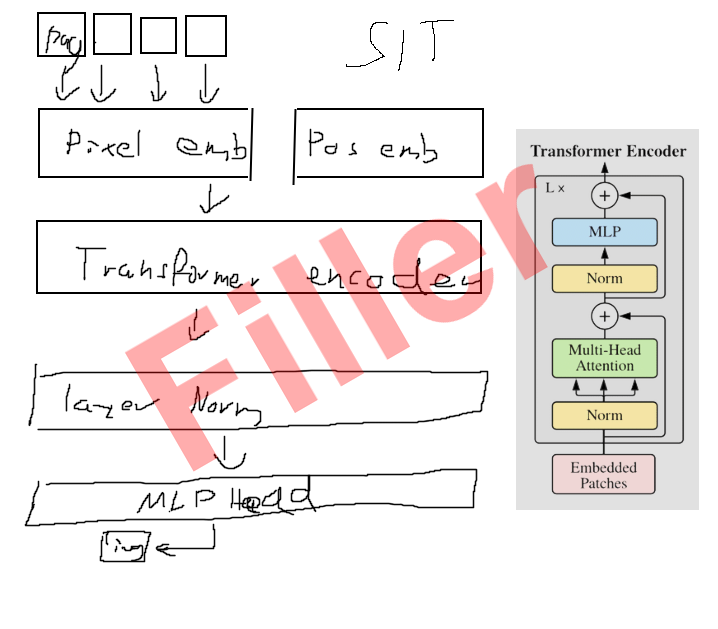
\includegraphics[width=0.8\textwidth]{imgs/SITModel.png}
        \caption{Spiral Image Transformer Model}
        \label{fig:SpiralImageTransformer}
    \end{figure}

    The visual representation above illustrates the operational steps of the SIT model. Similar to the CIT model, it begins by loading and converting the data. However, it diverges in its method by transforming the data into a spiral format, instead of using the columnar approach employed by the CIT. Like its counterpart, this model embeds pixels, from 3 colors to a higher-dimensional embedding space represented by \(N_{\text{EMBD}}\). Positional embeddings are then added. The embedded data is further processed by a (MLP), which converts it back into the original 3-color format. Finally, the spiral-formatted data is restructured into the original image layout.

    \subsubsection{Spiral Data Processing}

    To transform the data, which is loaded by the DataLoader and iterated over, into a spiral format, the width and height dimensions are first squeezed into a single dimension. This resulting tensor has the shape (Batch, Color Channels, Spiral Length). The next step involves indexing the data into the spiral form. For more detailed information on this indexing process, refer to \autoref{fig:spiral_indexing_1}. The restructured tensor is then processed like how the data is handled in the Column Image Transformer. The following code block illustrates the process used to convert the data into a spiral format.

    \begin{figure}[H]
        \centering
        \begin{lstlisting}[language=Python]
def get_batch(data):
    # Batch_size, Color Channels, Height, Width
    B, C, H, W = data.shape

    spiral_data = torch.zeros_like(data.view(B, C, -1))

    spiral_data[:,:,spiral_indices.flatten()] = data.view(B, C, -1)

    source = spiral_data[:, :, :BLOCK_SIZE]
    label = spiral_data[:, :, 1:BLOCK_SIZE+1]

    source = rearrange(source, 'b c h -> b h c')
    label = rearrange(label, 'b c h -> b h c')

    return source, label
        \end{lstlisting}
        \caption{Get data in a spiral form for the SIT model}
        \label{fig:spiral_indexing_code}
    \end{figure}

    \subsubsection{Spiral generation}
    \label{sec:spiral_generation}
    The conversion of data into a spiral form needs to be highly efficient because the code block will execute for every training step. Therefore, a simple nested for loop is insufficient to rearrange the data into the desired form. In this example, fancy indexing is used to convert the data into a spiral form. Thus, the data tensor is indexed with a flattened two-dimensional tensor containing the indices of the spiral form.

    At the start of the model training script, one indexing spiral is created to be used for all images in the dataset. The following code block illustrates the creation of the spiral index tensor.

\begin{figure}[H]
\centering
\begin{lstlisting}[language=Python]
def create_spiral(n): # n = width and height
    
    matrix = [[0] * n for _ in range(n)] # Initialize n x n matrix

    x, y = 0, 0
    # Direction vectors (right, down, left, up)
    dx = [0, 1, 0, -1]
    dy = [1, 0, -1, 0]
    direction = 0

    for i in range(n * n - 1, -1, -1):  # Start (35 for 6x6)
        matrix[x][y] = i
        nx = x + dx[direction]
        ny = y + dy[direction]

        # Change direction if the next position: out of bounds or filled
        if nx<0 or nx>=n or ny<0 or ny>=n or matrix[nx][ny]!=0:
            direction = (direction + 1) % 4  # Change direction
            nx = x + dx[direction]
            ny = y + dy[direction]

        x, y = nx, ny
    
    return torch.tensor(matrix)
\end{lstlisting}
\caption{Python function to create a spiral index tensor}
\label{fig:spiral_matrix}
\end{figure}

    The code above generates a square matrix of size n by n, then fills it with numbers in a spiral pattern, starting from the outer edge and spiraling inwards clockwise. Each cell of the matrix is assigned a unique number, beginning from the highest value in the top-left corner and decreasing by one with each step along the spiral path until reaching zero at the center or the end of the spiral. The spiral formation is achieved by moving right, then down, then left, then up, and repeating this sequence, adjusting direction whenever the next step would go out of bounds or into a cell that's already been filled.

    The generated spiral index tensor is then used to index the data tensor, effectively converting it into a spiral form. The following image illustrates the process of converting a 7x7 image.
    
    
    \begin{figure}[H]
    \centering
    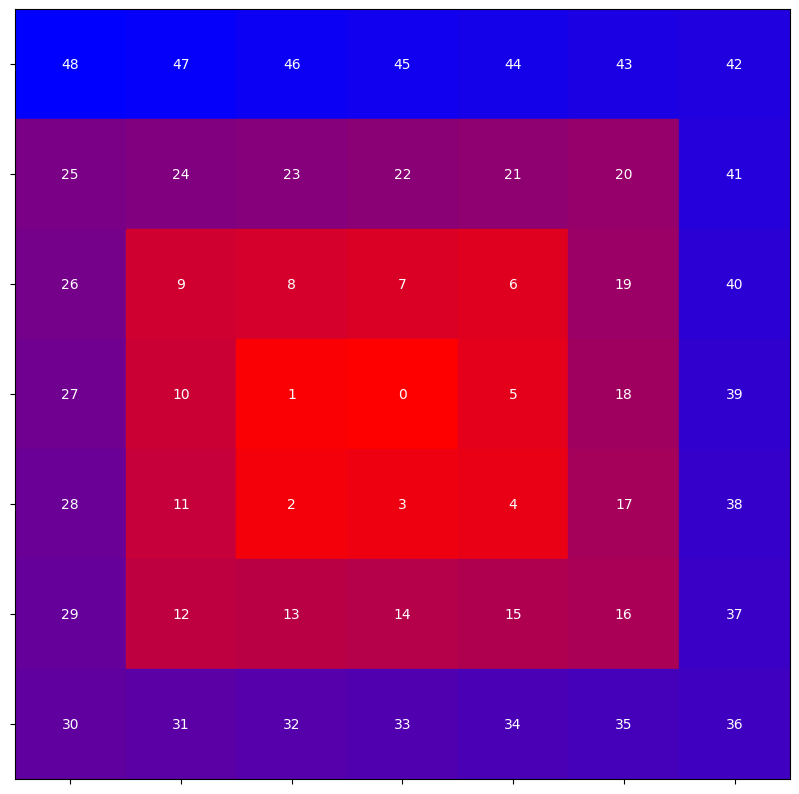
\includegraphics[width=0.6\textwidth]{../code/dataAnalysis/plots/exampleImgs/spiralShowcase1.png}
    \caption{Image representation}
    \label{fig:spiral_indexing_1}        
    \end{figure}

    \begin{figure}[H]
    \centering
    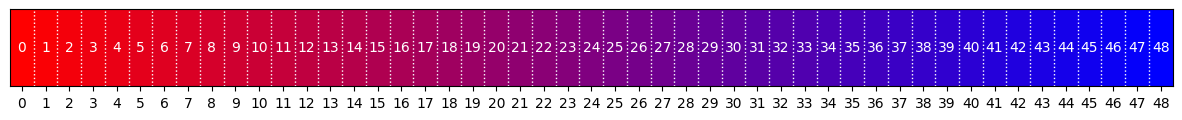
\includegraphics[width=1\textwidth]{../code/dataAnalysis/plots/exampleImgs/spiralShowcase0.png}
    \caption{7x7 Image flattened into a spiral form} 
    \label{fig:spiral_indexing_0}        
    \end{figure}

    As shown in \autoref{fig:spiral_indexing_1}, the pixels of the image are labeled with their respective indices 0, \dots, 43. The image is then unrolled into a single dimension, as shown in \autoref{fig:spiral_indexing_0}. The centering pixel is the first element of the spiral, and the spiral continues counterclockwise from there. In the model script, the dimensions for width and height typically exceed a width of 7, yet the underlying process remains unchanged.



\subsubsection{Model Architecture}

Similar to the CIT model, the addition of positional embeddings is handled in the same manner. This is because the data is transformed into a spiral pattern, allowing the addition of positional embeddings to remain unchanged. Additionally, the transformer layer operates identically. For more information on the transformer layer, see the CIT model \autoref{sec:transformer_CIT}.


\subsubsection{Training the Model}
2.3.5 Training Protocols
Discuss the training process, highlighting any unique considerations for the spiral data format.

2.3.6 Optimization and Loss Functions
Specific optimization techniques and loss functions that are effective for spiral-based models.

\subsubsection{Experimental Results}
Multiple experiments are conducted to evaluate the performance of the SIT model. The experiments are designed to test the models ability to generate images, the quality of the generated images, and the models performance on different datasets. The results are analyzed to identify the strengths and weaknesses of the model.

In each of the tests, the end of the seed pixels is marked with a purple line on the left side of the image.

    \begin{itemize}
        \item \textbf{Color test:} To test the models capability to generate certain colors the model is given a test image with one single color filling the whole context. Then the model generates the next flowing 32 pixels. 
        
        %TODO: 
        TODO: Add color test images models output

        \item \textbf{Zebra pattern test:} The second test is to see if the model is capable of generating a zebra pattern. The model is given a vertical and a horizontal test image with a black and white colored zebra pattern with a pixel width of 3. The model then generates the next 32 pixels.
        
        %TODO:
        TODO: Add zebra pattern test images models output

        \item \textbf{Spiral Pattern test:} The third test is to see if the model is capable of generating a full image. The model is given a test image with a 4x4 pixel pattern. The model then generates the next 32 pixels.
    \end{itemize}


\subsubsection{Challenges and Limitations}
2.3.9 Identified Challenges
Discuss specific challenges encountered during the development and implementation phases.

2.3.10 Limitations of the Spiral Transformer
Critically analyze the limitations and potential drawbacks of using a spiral approach.